%package list
\documentclass{article}
\usepackage[top=3cm, bottom=3cm, outer=3cm, inner=3cm]{geometry}
\usepackage{graphicx}
\usepackage{url}
%\usepackage{cite}
\usepackage{hyperref}
\usepackage{array}
\usepackage{multicol}
\newcolumntype{x}[1]{>{\centering\arraybackslash\hspace{0pt}}p{#1}}
%\usepackage{natbib}
\usepackage{pdfpages}
\usepackage{multirow}
\usepackage{float}
\usepackage[normalem]{ulem}
\useunder{\uline}{\ul}{}

\usepackage{listings}
\usepackage{xcolor}
\usepackage{algorithm,algorithmic}

\usepackage{caption}
\usepackage{subcaption}


\definecolor{codegreen}{rgb}{0,0.6,0}
\definecolor{codegray}{rgb}{0.5,0.5,0.5}
\definecolor{codepurple}{rgb}{0.58,0,0.82}
\definecolor{backcolour}{rgb}{0.95,0.95,0.92}

\lstdefinestyle{style_code}{
    backgroundcolor=\color{backcolour},   
    commentstyle=\color{codegreen},
    keywordstyle=\color{magenta},
    numberstyle=\tiny\color{codegray},
    stringstyle=\color{codepurple},
    basicstyle=\ttfamily\footnotesize,
    breakatwhitespace=false,         
    breaklines=true,                 
    captionpos=b,                    
    keepspaces=true,                 
    numbers=left,                    
    numbersep=5pt,                  
    showspaces=false,                
    showstringspaces=false,
    showtabs=false,                  
    tabsize=2
}

\usepackage{color}
\definecolor{lightgray}{rgb}{.9,.9,.9}
\definecolor{darkgray}{rgb}{.4,.4,.4}
\definecolor{purple}{rgb}{0.65, 0.12, 0.82}

\lstdefinelanguage{JavaScript}{
  keywords={typeof, new, true, false, catch, function, return, null, catch, switch, var, if, in, while, do, else, case, break},
  keywordstyle=\color{blue}\bfseries,
  ndkeywords={class, export, boolean, throw, implements, import, this},
  ndkeywordstyle=\color{darkgray}\bfseries,
  identifierstyle=\color{black},
  sensitive=false,
  comment=[l]{//},
  morecomment=[s]{/*}{*/},
  commentstyle=\color{purple}\ttfamily,
  stringstyle=\color{red}\ttfamily,
  morestring=[b]',
  morestring=[b]"
}

\lstset{
   language=JavaScript,
   backgroundcolor=\color{lightgray},
   extendedchars=true,
   basicstyle=\tiny\ttfamily,
   %basicstyle=\footnotesize\ttfamily,
   showstringspaces=false,
   showspaces=false,
   numbers=left,
   numberstyle=\footnotesize,
   numbersep=4pt,
   tabsize=1,
   breaklines=true,
   showtabs=false,
   captionpos=b
}

\lstset{style=style_code}

%%% para algorithm
%\floatname{algorithm}{Procedure}
\renewcommand{\algorithmicrequire}{\textbf{Input:}}
\renewcommand{\algorithmicensure}{\textbf{Output:}}

%%%%%%%%%%%%%%%%%%%%%%%%%%%%%%%%%%%%%%%%%%%%%%%%%%%%%%%%%%%%%%%%%%%%%%%%%%%%
%%%%%%%%%%%%%%%%%%%%%%%%%%%%%%%%%%%%%%%%%%%%%%%%%%%%%%%%%%%%%%%%%%%%%%%%%%%%
\newcommand{\csemail}{vmachacaa@unsa.edu.pe}
\newcommand{\csdocente}{Vicente Machaca Arceda}
\newcommand{\cscurso}{Estructura de Datos y Algoritmos}
\newcommand{\csuniversidad}{Universidad Nacional de San Agustín}
\newcommand{\csescuela}{Maestría en Ciencia de la Computación}
\newcommand{\cspracnr}{04}
\newcommand{\cstema}{Kd-Tree}
%%%%%%%%%%%%%%%%%%%%%%%%%%%%%%%%%%%%%%%%%%%%%%%%%%%%%%%%%%%%%%%%%%%%%%%%%%%%
%%%%%%%%%%%%%%%%%%%%%%%%%%%%%%%%%%%%%%%%%%%%%%%%%%%%%%%%%%%%%%%%%%%%%%%%%%%%


\usepackage[english,spanish]{babel}
\usepackage[utf8]{inputenc}
\AtBeginDocument{\selectlanguage{spanish}}
\renewcommand{\figurename}{Figura}
\renewcommand{\refname}{Referencias}
\renewcommand{\tablename}{Tabla} %esto no funciona cuando se usa babel
\AtBeginDocument{%
	\renewcommand\tablename{Tabla}
}

\usepackage{fancyhdr}
\pagestyle{fancy}
\fancyhf{}
\setlength{\headheight}{30pt}
\renewcommand{\headrulewidth}{1pt}
\renewcommand{\footrulewidth}{1pt}
\fancyhead[L]{\raisebox{-0.2\height}{
\includegraphics[width=3cm]{img/logo_unsa}}}
\fancyhead[C]{}
\fancyhead[R]{\fontsize{7}{7}\selectfont	\csuniversidad \\ \csescuela \\ \textbf{\cscurso} }
\fancyfoot[L]{MSc. Vicente Machaca}
\fancyfoot[C]{\cscurso}
\fancyfoot[R]{Página \thepage}

\begin{document}
	
	\vspace*{10px}
	
	\begin{center}	
		\fontsize{17}{17} \textbf{ Práctica \cspracnr}
	\end{center}
	%\centerline{\textbf{\underline{\Large Título: Informe de revisión del estado del arte}}}
	%\vspace*{0.5cm}
	

	\begin{table}[h]
		\begin{tabular}{|x{4.7cm}|x{4.8cm}|x{4.8cm}|}
			\hline 
			\textbf{DOCENTE} & \textbf{CARRERA}  & \textbf{CURSO}   \\
			\hline 
			\csdocente & \csescuela & \cscurso    \\
			\hline 
		\end{tabular}
	\end{table}	
	
	
	\begin{table}[h]
		\begin{tabular}{|x{4.7cm}|x{4.8cm}|x{4.8cm}|}
			\hline 
			\textbf{PRÁCTICA} & \textbf{TEMA}  & \textbf{DURACIÓN}   \\
			\hline 
			\cspracnr & \cstema & 3 horas   \\
			\hline 
		\end{tabular}
	\end{table}
	
	
	\section{Datos de los estudiantes}
	\begin{itemize}
		\item Grupo: 9
		\item Integrantes: 
		\begin{itemize}
			\item Abarca Murillo, Jhonatan Piero
			\item Apari Pinto, Christian Timoteo
			\item Suca Velando, Christian Anthony
			\item Vargas Zuni, Arturo
		\end{itemize}
		\item Repositorio: \url{https://github.com/jabarcamu/EDA_Practica4}
		\item Video: \url{https://youtu.be/2EECiQbAocA}
	\end{itemize}
	
	

	
	\section{Ejercicios}\label{sec:ejercicios}
	
	    \subsection{Cree un archivo \textit{main.html}} 
		
		\lstinputlisting[language=HTML, firstline=2, lastline=11, caption=index.html]{code/index.html}
		
		La distribucion de los archivos se mantienen por carpetas, en la carpeta js se tienen los archivos javascript ejecutables , tanto del arbol kdtree como del graficador usando la libreria p5.js, en la carpeta css los estilos que manejará, en este caso se optó por la libreria bootstrap. 
		
		
		\subsection{Cree un archivo \textit{kdtree.js}} 
		
		A medida que va aumentado la dimensión del espacio $d$, como por ejemplo el número de atributos, cada nivel de descomposicion del quadtree resulta en muchas nuevas celdas o cuadrantes mientras vamos aumentando la dimension llegando a ser muy alta, por ejemplo $2^n$. Esta situacion es mitigada haciendo uso de variantes de un $k-d tree$, en el que $k$ demota la dimensionalidad de el espacio a ser representado, si embargo en muchas aplicaciones la convension llega a ser que el valor de $d$ denota la dimension, y esto es en la practica el camino que elegimos seguir. En principio $kd-tree$ es un arbol binario donde el espacio subyaciente es particionado en la base del valor de solo un atributo en cada nivel del árbol en lugar de la base de los valores $d$ como en el caso de Quadtree. En otras palabras, la distinción con Quadtree es que en $kd-Tree$ solo un atributo, o la clave, es evaluado cuando determina la dirección en que cada rama sera hecha  \cite{Morgan2006}.
        
        \begin{figure}[H]
			\centering
			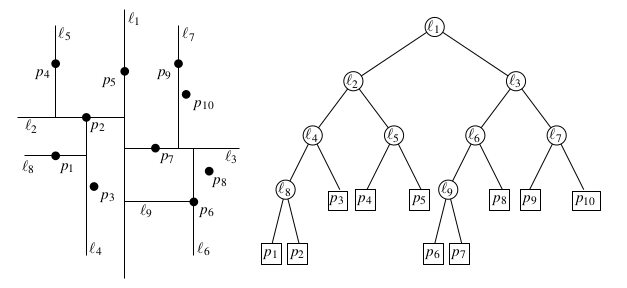
\includegraphics[scale=0.40]{img/kdtree1.png}
			\caption{kd-Tree  \cite{compgeom:2000}}
			\label{fig:kdtree1}
		\end{figure}		
		
		Originalmente el nombre se entiende como un arbol de $k-$dimensiones; tomando un ejemplo, el generar un arbol de 2-dimensiones será llamado como un $2d-tree$  \cite{compgeom:2000}, originalmente este término a sido olvidado actualmente solamente se conoce como 2-dimensiones kd-tree como se muestra en la figura \ref{fig:kdtree1}.
		
		Para la construcción del $kd-tree$ sera a partir de las siguientes características mostradas en el siguiente código. Un atributo punto (point) que almacena el punto en la k-dimensión, puntero a la izquierda (left) apuntador a la generacion del hijo izquierdo, puntero a la derecha y finalmente el eje al que actualmente se estara evaluando, en la parte de la construcción del kd-tree se explica con mayor detalle.
		
		\lstinputlisting[language=JavaScript, firstline=4, lastline=11, caption=kdtree.js]{code/kdtree.js}
		
		\subsection{Complete las funciones}
		    
		    \subsubsection{build kdtree: Construye el KD-Tree y retorna el nodo raiz.} 
		    
		        Podemos construir un $kd-tree$ con un procedimiento recursivo que se describe a continuación.\\
                Este procedimiento tiene dos parámetros: un conjunto de puntos y un número entero. El primer parámetro es el conjunto para el que queremos construir el $kd-tree$, inicialmente esta es el conjunto P. El segundo parámetro es la profundidad de recursividad o, en otras palabras, la profundidad de la raíz del subárbol que construye la llamada recursiva. El parámetro de profundidad es cero en la primera llamada. La profundidad es importante porque determina si debemos partir con una línea vertical u horizontal. El procedimiento devuelve la raíz del $kd-tree$ \cite{compgeom:2000}.
    		    
    		    \lstinputlisting[language=JavaScript, firstline=53, lastline=78, caption=buildKdtree]{code/kdtree.js}
    		    
    		\subsubsection{getHeight: Retorna la altura del árbol} 
    		    
    		    Verifica si el árbol no esta vacio, luego recursivamente retornamos la altura del nodo izquierdo y derecho, respecto al valor que estamos por recibir tanto de la altura izquierda y derecha comparamos si dicha altura es mayor en una de las ramas, así tomar como altura del árbol al lado mayor según la comparación realizada
    		    
    		    \lstinputlisting[language=JavaScript, firstline=13, lastline=32, caption=getHeight]{code/kdtree.js}
    		    
    		 \subsubsection{generate dot: Genera al árbol en formato dot} 
    		 
    		    Este procedimiento es similar al encontrar la altura del árbol, con la diferencia que solamente requerimos solamente imprimir el punto padre que este apuntando a un hijo recursivamente para luego obtener el resultado mediante el graficador Graphviz de Python.
    		    
    		    \lstinputlisting[language=JavaScript, firstline=34, lastline=51, caption=generateDot]{code/kdtree.js}
		
		\subsection{Cree un archivo \textit{sketch.js}  y evalue sus resultados} 
		
		    Utilizando la librería gráfica p5.js, iniciaremos el dibujo general de los puntos 800x800 para que la generación se tenga mayor visibilidad de los puntos generados en adelante, en este caso solo se uso la dimensión de 500x500, y para la generación de los puntos se utilizo la variable $particleCount$ para generar los puntos aleatorios, para este caso ejemplo se tomaran 100 puntos aleatorios, finalmente la generación de cada punto esta dimensionada por una grilla interna para distinguir los sectores de separación de los puntos como se muestra en la figura \ref{fig:sketch1}
		    
		    \begin{figure}[H]
    			\centering
    			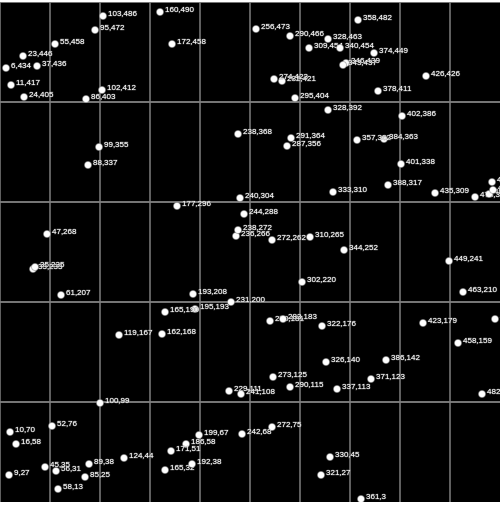
\includegraphics[scale=0.40]{img/sketch1.png}
    			\caption{sketch.js, dibujando los puntos}
    			\label{fig:sketch1}
    		\end{figure}
    		
    		Respecto a los puntos generados aleatoriamente, para el caso mostrado en el siguiente codigo, la dimension de los puntos es de 2-dimensiones y iniciamos el arbol llamando a la funcion $build_kdtree$ pasando como parámetros a los puntos generados, ver figura \ref{fig:sketch2}.
    		
    		\begin{figure}[H]
    			\centering
    			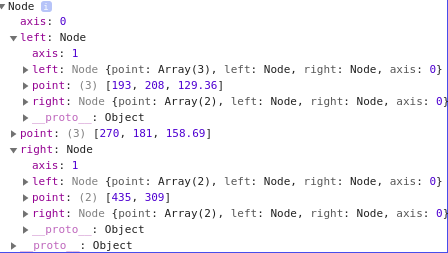
\includegraphics[scale=0.40]{img/sketch2.png}
    			\caption{sketch.js, iniciando el $kd-tree$}
    			\label{fig:sketch2}
    		\end{figure}
    		
		    \lstinputlisting[language=JavaScript, firstline=5, lastline=33, caption=sketch.js]{code/sketch.js}
		    
		    Así mismo ya creado el $kd-tree$ empezaria a llamarse a las otras funciones iniciales como la funcion $getHeight$ que devuelve 
		    
		    \begin{verbatim}
		        Altura del Arbol es 7
		    \end{verbatim}
		    
		    Finalmente el resultado de los puntos desde generateDot para graficarlos en GraphViz, como se ve en la figura \ref{fig:sketch3}
		    
		    \begin{figure}[H]
    			\centering
    			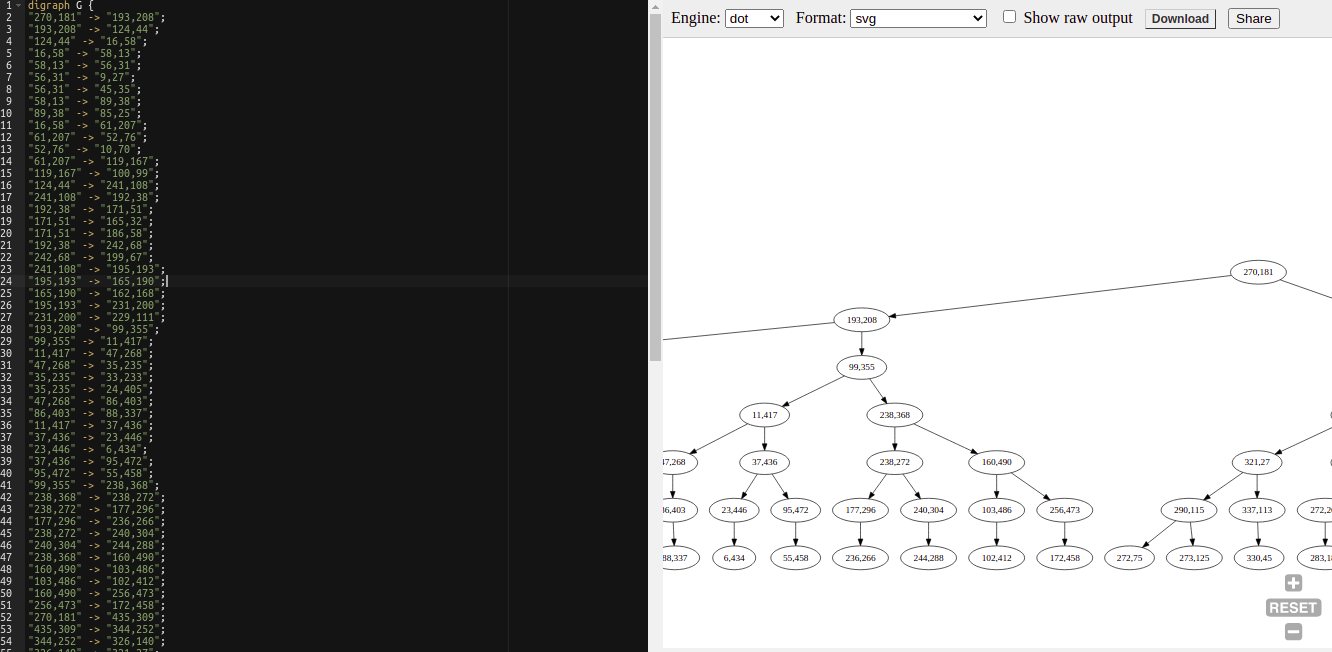
\includegraphics[scale=0.35]{img/sketch3.png}
    			\caption{sketch.js, resultado de $generate\_dot$}
    			\label{fig:sketch3}
    		\end{figure}
		    
		    
		\subsection{Implemente la función closest point brute force y naive closest point}
		
		    Previamente para generar los dos siguientes algoritmos se requiere de la creación de la función de distancia Euclidiana o cuadrática, se define la siguiente función que recibe como parámetros dos puntos de la misma dimensión y calcula su distancia en ellas como se muestra en el siguiente código.
		    
		    \lstinputlisting[language=JavaScript, firstline=80, lastline=89, caption=distanceSquared]{code/kdtree.js}
		
    	    \subsubsection{Closest point brute force}
    	        
    	        Respecto para realizar la búsqueda por fuerza bruta es directamente comparar el punto a consultar con todos los puntos existentes en la lista completa generada, no se requiere de la iniciación de la estructura $kd-tree$ sino que realiza el cálculo de las distancias clasificando la distancia menor cada vez que se realiza una comparación la distancia actual se toma como la mejor hasta que vaya recorriendo en todos los puntos hasta el final clasificando solamente el punto más próximo. El rendimiento del algoritmo es el mas ineficiente ya que requiere realizar comparaciones con todos los puntos.
    	        
    	        \lstinputlisting[language=JavaScript, firstline=91, lastline=102, caption=closestPointBruteForce]{code/kdtree.js}
    	        
    	    \subsubsection{Naive closest point} 
    	    
    	        Para la definición de esta función se requiere del ingreso del $kd-tree$, el punto a consultar y directamente ya se va actualizando la profundidad del árbol mientras va realizando su recorrido tomando su mejor resultado. Para este proceso siempre tomando el nodo actual desde el padre hacia los hijos, claramente tiene el mismo comportamiento del que se espera del binary tree, en este caso inicia tomando su primera dimensión, ya que solamente tenemos 2-dimensiones esta sera la X, luego realiza la consulta respecto a la misma dimensión del punto hacia donde tiene que dirigirse la consulta, actualizando el mejor nodo siempre con respecto al eje al que se consulta en su profundidad (va permutando realizando la consulta mediante la operación módulo $\%$), finalmente si se eligió el camino correcto a seguir nuevamente se llama a la función principal recursivamente hasta encontrar el ultimo hijo respecto a la consulta. La contra de este algoritmo es que puede ser que el punto en realidad esta mas próximo en alguno de los ejes padre aun siendo este algoritmo mas eficiente con respecto al anterior 
    	        \lstinputlisting[language=JavaScript, firstline=104, lastline=121, caption=naiveClosestPoint]{code/kdtree.js}
        	
		
		\subsection{Evalúe el resultado de las dos funciones implementadas anteriormente con este conjunto de datos} 
		    \begin{verbatim}
		        var data = [
                [40 ,70] ,
                [70 ,130] ,
                [90 ,40] ,
                [110 , 100] ,
                [140 ,110] ,
                [160 , 100]
                ];
                var point = [140 ,90]; // query
		    \end{verbatim}  
		    
		    Tomando ventaja de la función que grafica los puntos y la herramienta GraphViz se muestra en la figura \ref{fig:query1}
		    
		    \begin{figure}[H]
    			\centering
    			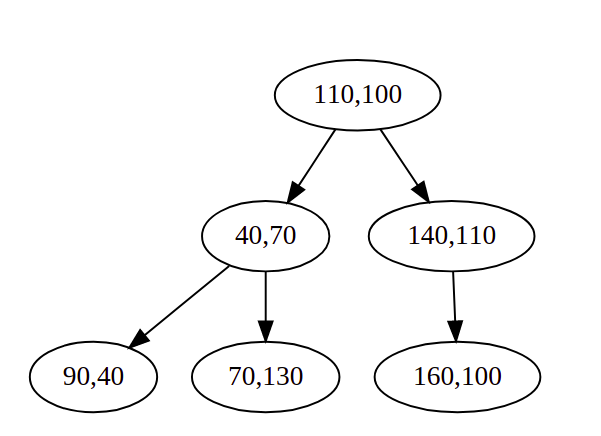
\includegraphics[scale=0.35]{img/query1.png}
    			\caption{Vista GraphViz}
    			\label{fig:query1}
    		\end{figure}
		
		    %%% aqui deberia ir con sustento grafico mas
		    
		    Como se muestra en figura los resultados directos desde realizar la búsqueda del punto mas cercano utilizando la fuerza bruta da como resultado el punto verdaderamente más cercano pero con un rendimiento mayor, $closest\_point\_brute\_force$ directamente devuelve el resultado con respecto al acumulado en cada punto consultado. En cambio $naive\_closest\_point$ va realizando las consultas de que lado del hijo se ira, en este caso tomara el lado derecho y seguirá recursivamente hasta hallar el hijo del total de la altura del árbol, tomando a este como el resultado final, siendo erróneo ya que el mínimo es su padre anterior a el por su cercanía al punto tal como se muestra en la figura \ref{fig:query2}.
		    
		    \begin{figure}[H]
    			\centering
    			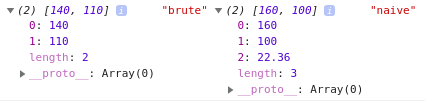
\includegraphics[scale=0.45]{img/query2_result.png}
    			\caption{Resultado de ambos algoritmos de búsqueda del punto con menor distancia}
    			\label{fig:query2}
    		\end{figure}
		    
		    
		
		\subsection{Evalúe el resultado de las dos funciones implementadas anteriormente con este conjunto de datos} 
		
		%% aqui deberia ir con sustento grafico mas
		    \begin{verbatim}
		        var data = [
                [40 ,70] ,
                [70 ,130] ,
                [90 ,40] ,
                [110 , 100] ,
                [140 ,110] ,
                [160 , 100] ,
                [150 , 30]
                ];
                var point = [140 ,90]; // query
		    \end{verbatim} 
		    
		    Tomando ventaja de la función que grafica los puntos y la herramienta GraphViz se muestra en la figura \ref{fig:query3}
		    
		    \begin{figure}[H]
    			\centering
    			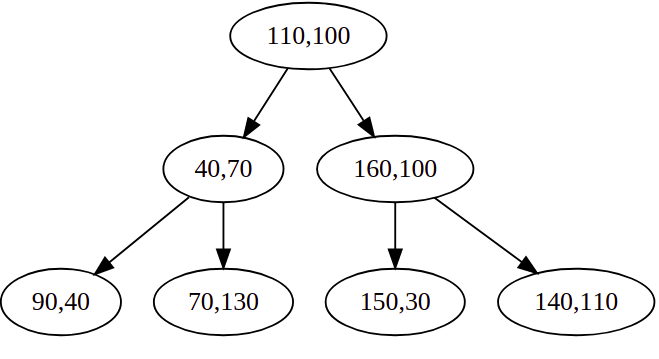
\includegraphics[scale=0.35]{img/query3.png}
    			\caption{Vista GraphViz 2}
    			\label{fig:query3}
    		\end{figure}
    		
    		$closest\_point\_brute\_force$ al igual que en el anterior caso, directamente devuelve el resultado con respecto al acumulado en cada punto consultado encontrando al punto con la distancia mas cercana al anterior. En cambio $naive\_closest\_point$ va realizando las consultas de que lado del hijo se ira, en este caso tomara el lado derecho y seguirá recursivamente hasta hallar el hijo del total de la altura del árbol aun habiendole aumentado un punto mas el cual acercaria mas su resultado pero el punto padre es el mas cercano dejando a este punto fuera del rango de respuesta próximo tal como se muestra en la figura \ref{fig:query4_result}.
    		
    		\begin{figure}[H]
    			\centering
    			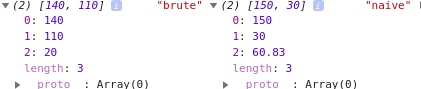
\includegraphics[scale=0.45]{img/query4_result.png}
    			\caption{Resultado del segundo conjunto de puntos con los algoritmos presentados}
    			\label{fig:query4_result}
    		\end{figure}
		
		\subsection{Ahora implemente la función closest point, siguiendo las recomendaciones dadas por el docente} 
		
		    Como mejora a la función $naive\_closest\_point$ se realiza el cálculo de la distancia mas próxima durante la elección del punto mejor posicionado en el hijo donde se realizara la consulta, en este caso como ya se tiene previamente el mejor resultado el camino seguirá recorriendo tal cual como hacia pero el resultado se tomara respecto al punto que presento la distancia mas cercana al punto a consultar. 
		
		    \lstinputlisting[language=JavaScript, firstline=123, lastline=146, caption=closestPoint]{code/kdtree.js}
		    
		    Utilizando como ejemplo el mismo resultado del ultimo conjunto de datos presentado se tiene el verdadero resultado con la distancia más próxima al punto a consultar como se muestra en la figura \ref{fig:closest1}.
		    
		    \begin{figure}[H]
    			\centering
    			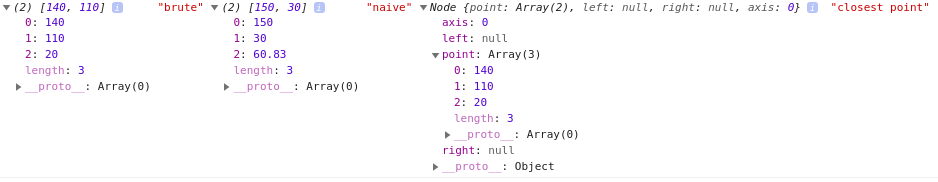
\includegraphics[scale=0.45]{img/closest1.png}
    			\caption{Mejora al algoritmo de búsqueda del punto más próximo a la consulta}
    			\label{fig:closest1}
    		\end{figure}
		
		\subsection{Averigue e implemente una función KNN, que retorna los k puntos mas cercanos a un punto} 
		    Antes de implementar el algoritmo k-nearest-neighbour se precisa obtener una función que calcule el resultado más cercano, el cual recibe como parámetro el punto de consulta, el punto al que se esta aproximando y el punto del padre.
		
    		\lstinputlisting[language=JavaScript, firstline=150, lastline=158, caption=masCercano]{code/kdtree.js}
    		
    	    Por consiguiente se define al algoritmo \cite{Morgan2006}:
    	    \begin{enumerate}
    	        \item Comenzando con el nodo raíz, el algoritmo se mueve hacia abajo en el árbol de forma recursiva, de la misma manera que lo haría si se estuviera insertando el punto de búsqueda (es decir, va hacia la izquierda o hacia la derecha dependiendo de si el punto es menor o mayor que el nodo actual en la dimensión).
    	        \item Una vez que el algoritmo llega a un nodo hoja, comprueba en ese punto de nodo si la distancia es mejor, ese punto de nodo se guarda como el mejor actual. (ver figura \ref{fig:knn_1_parte})
    	        \item El algoritmo desenrolla la recursividad del árbol, realizando los siguientes pasos en cada nodo:
    	            \begin{enumerate}
    	                \item Si el nodo actual está más cerca que el mejor actual, entonces se convierte en el mejor actual.
    	                \item El algoritmo verifica si podría haber puntos en el otro lado del plano de división que estén más cerca del punto de búsqueda que el mejor actual, se implementa una comparación simple para ver si la distancia entre la coordenada de división del punto de búsqueda y el nodo actual es menor que la distancia (coordenadas generales) desde el punto de búsqueda al mejor actual, en principio se definió la función de masCercano para realizar este proceso. Mientras el punto mas cercano sea menor al radio marcado entre la distancia del nodo anterior se tomara el siguiente hijo caso contrario se seguirá subiendo eliminando la rama que no cumple con el requisito (ver figura \ref{fig:knn_2_parte}).
    	            \end{enumerate}
    	        \item Cuando el algoritmo finaliza este proceso en el nodo raíz, la búsqueda está completa.
    	    \end{enumerate}
    	    
    	    \begin{figure}
             \centering
             \begin{subfigure}[b]{0.4\linewidth}
                 \centering
                 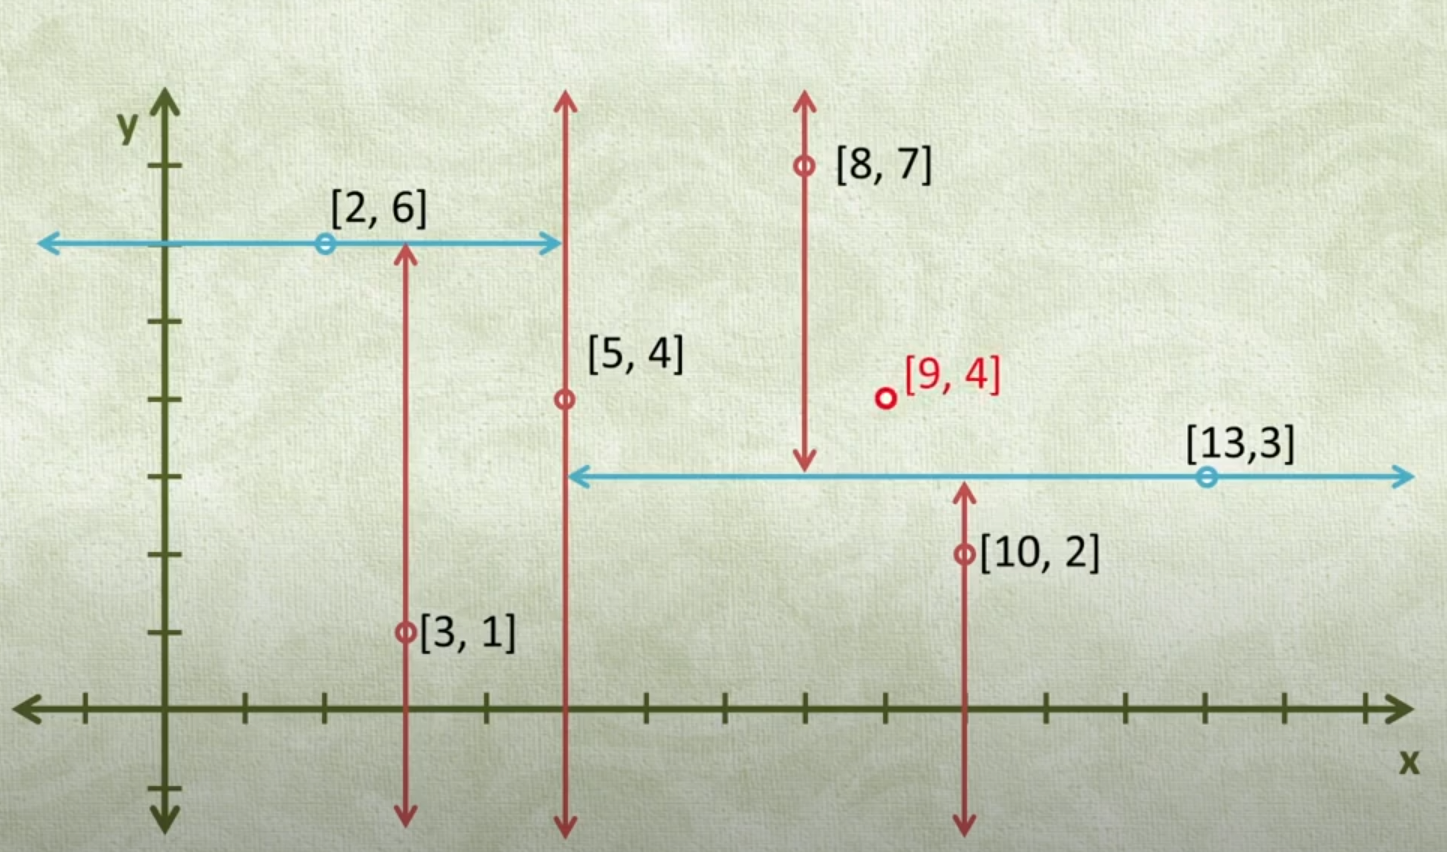
\includegraphics[width=\textwidth]{img/knn1.PNG}
                 \caption{El punto de consulta entra en el $kd-tree$}
                 \label{fig:knn1}
             \end{subfigure}
             \hfill
             \begin{subfigure}[b]{0.4\linewidth}
                 \centering
                 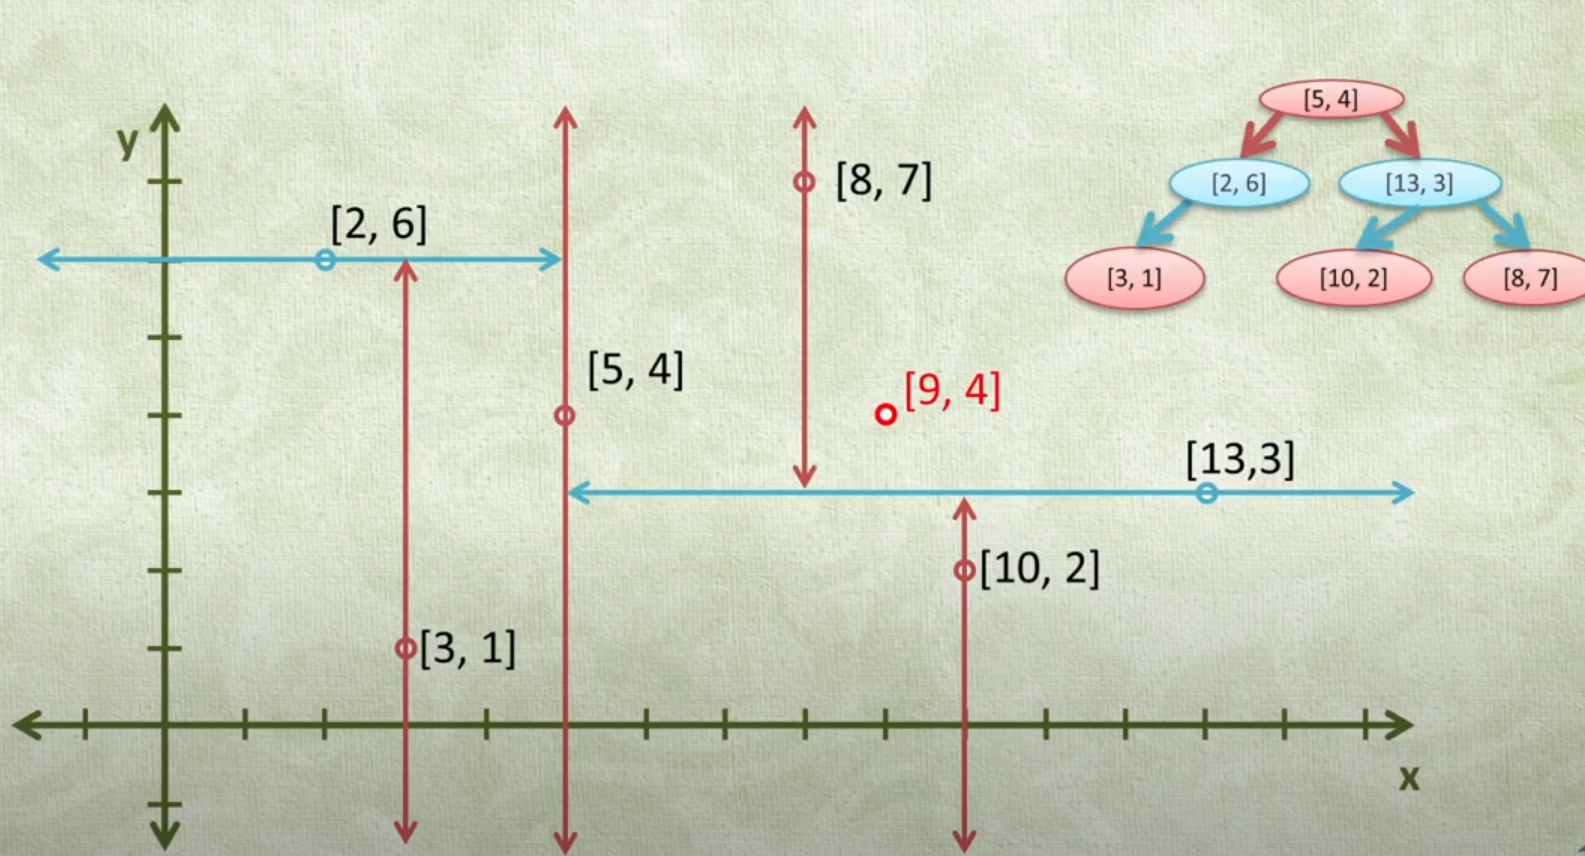
\includegraphics[width=\textwidth]{img/knn2.PNG}
                 \caption{Realizar la búsqueda desde la raíz hacia las hojas}
                 \label{fig:knn2}
             \end{subfigure}
             \hfill
             \begin{subfigure}[b]{0.4\linewidth}
                 \centering
                 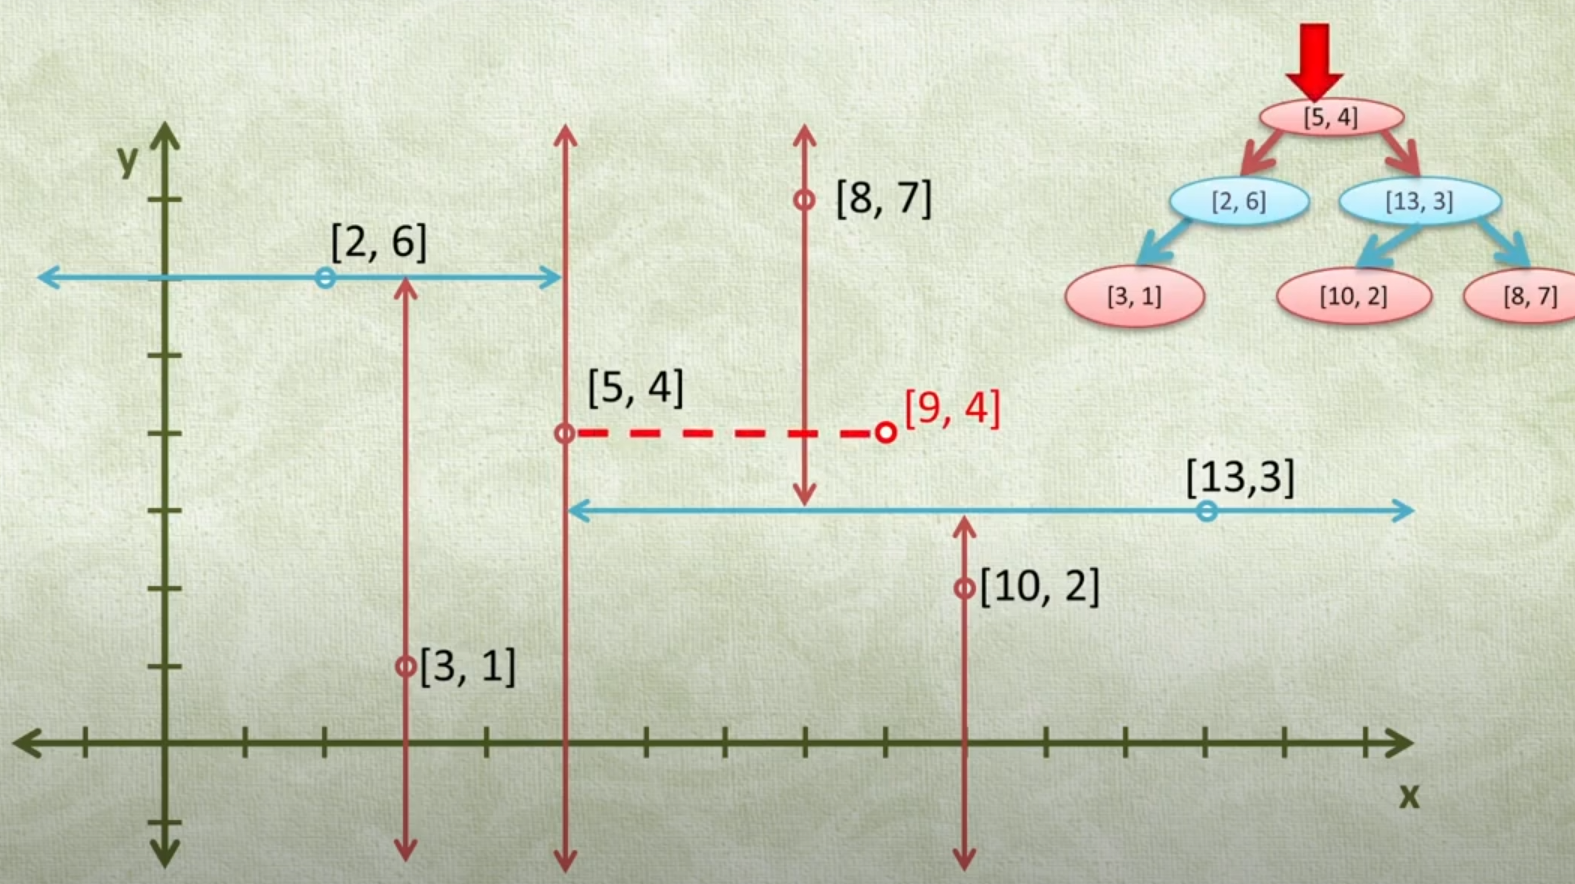
\includegraphics[width=\textwidth]{img/knn3.PNG}
                 \caption{Realiza la comparación de la distancia euclidiana sobre el nodo raíz}
                 \label{fig:knn3}
             \end{subfigure}
             \hfill
             \begin{subfigure}[b]{0.4\linewidth}
                 \centering
                 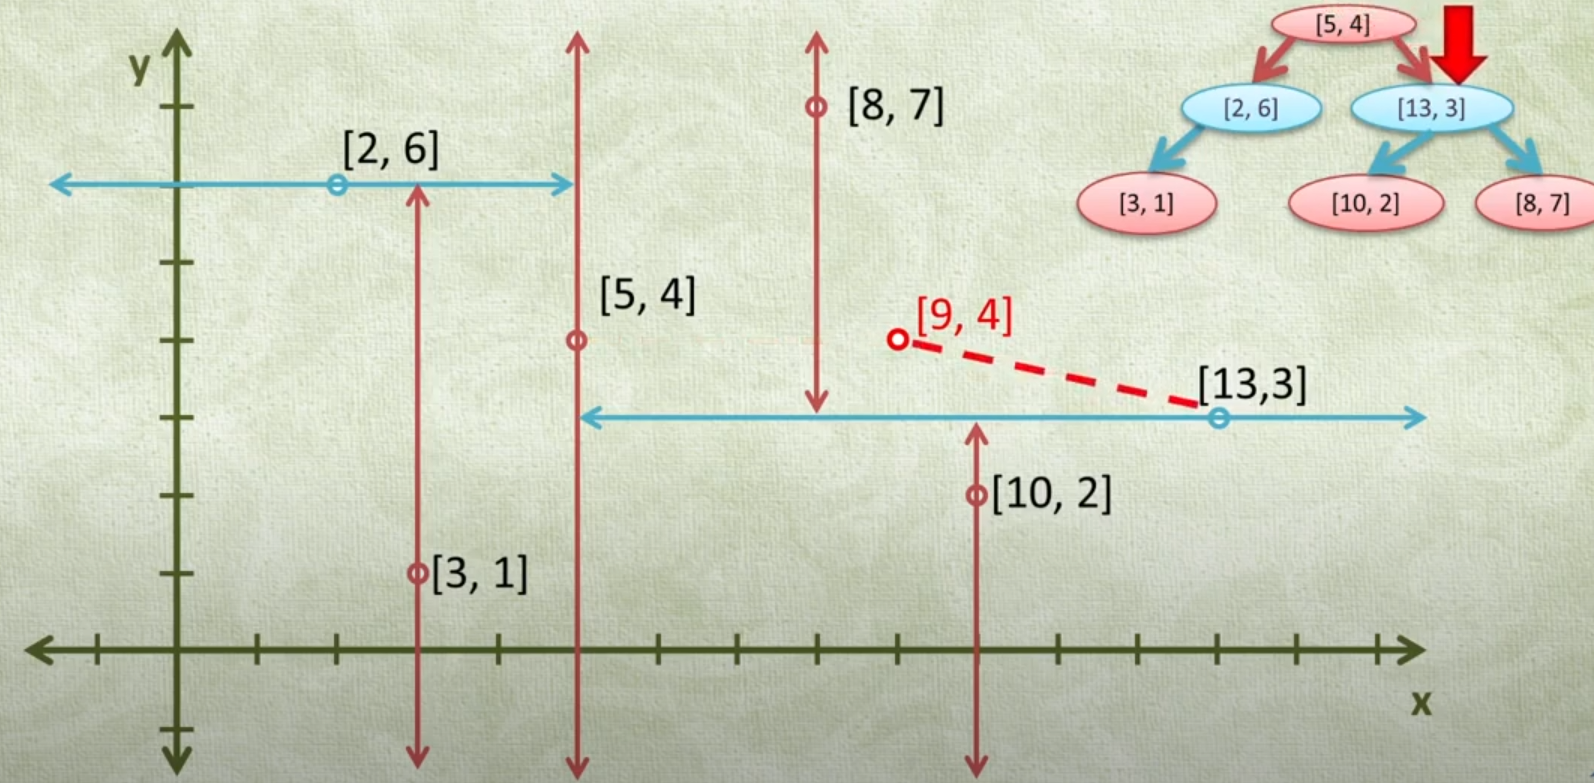
\includegraphics[width=\textwidth]{img/knn4.PNG}
                 \caption{Recorre el siguiente punto}
                 \label{fig:knn4}
             \end{subfigure}
                \caption{Ingreso de un nuevo punto a consultar}
                \label{fig:knn_1_parte}
            \end{figure}
            
            %%%%%%
            Al momento de repetir esta comparación tomará como máximo un tiempo de $O(2H)$ tomando H como la altura del árbol a recorrer, con esta condicional, la búsqueda en el árbol no realizara comparaciones con todos los puntos del árbol, puede solamente tomar $O(2H)$ como máximo de valores encontrados ordenados según su distancia.
            
            \begin{figure}
             \centering
             \begin{subfigure}[b]{0.4\linewidth}
                 \centering
                 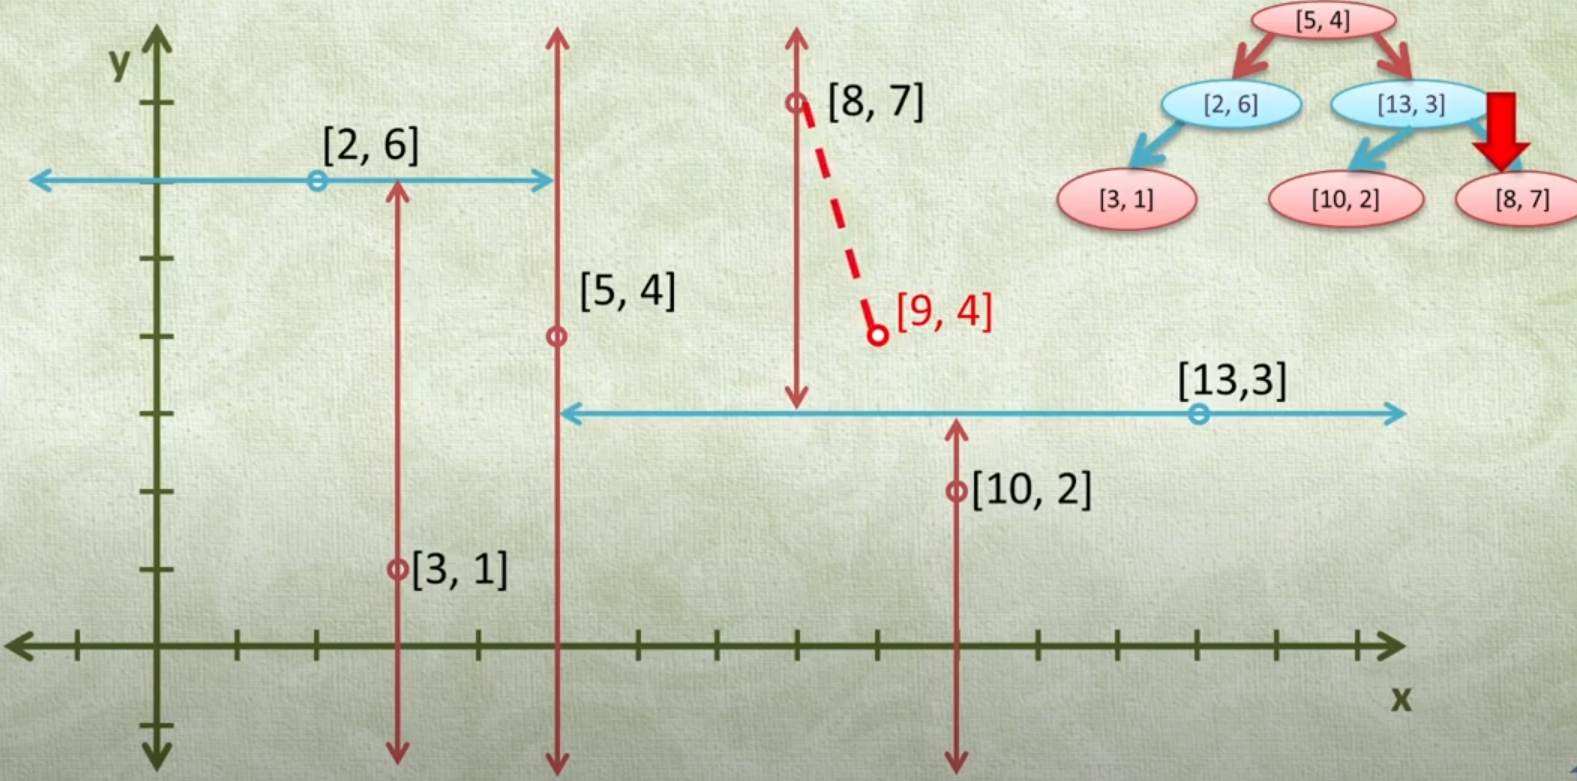
\includegraphics[width=\textwidth]{img/knn5.PNG}
                 \caption{Encuentra el ultimo punto de la rama del hijo mas próximo de la búsqueda}
                 \label{fig:knn5}
             \end{subfigure}
             \hfill
             \begin{subfigure}[b]{0.4\linewidth}
                 \centering
                 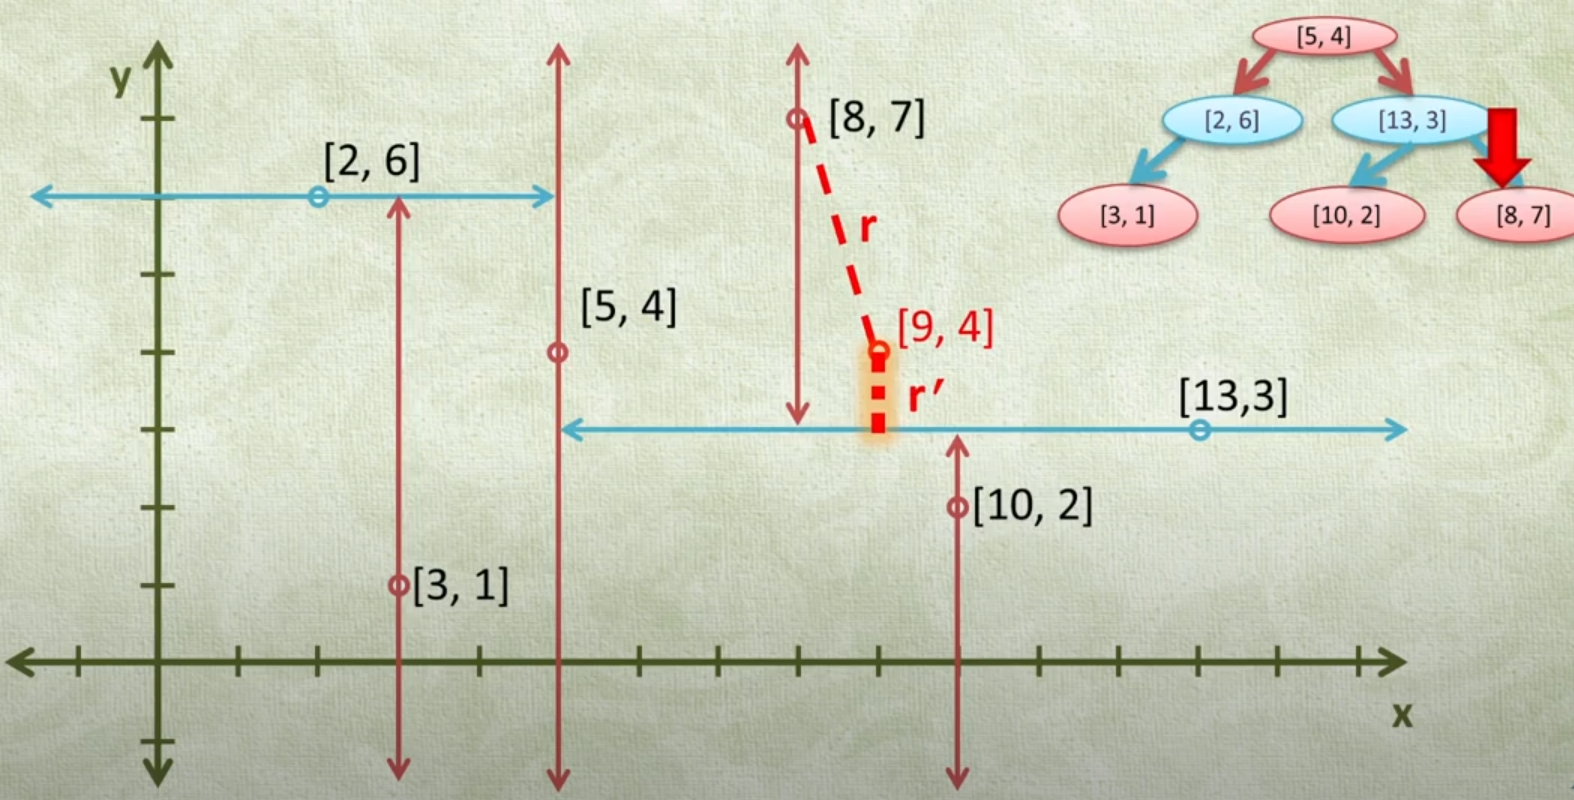
\includegraphics[width=\textwidth]{img/knn6.PNG}
                 \caption{La mejora del algoritmo, lo realiza desde retroceder recursivamente}
                 \label{fig:knn6}
             \end{subfigure}
             \hfill
             \begin{subfigure}[b]{0.4\linewidth}
                 \centering
                 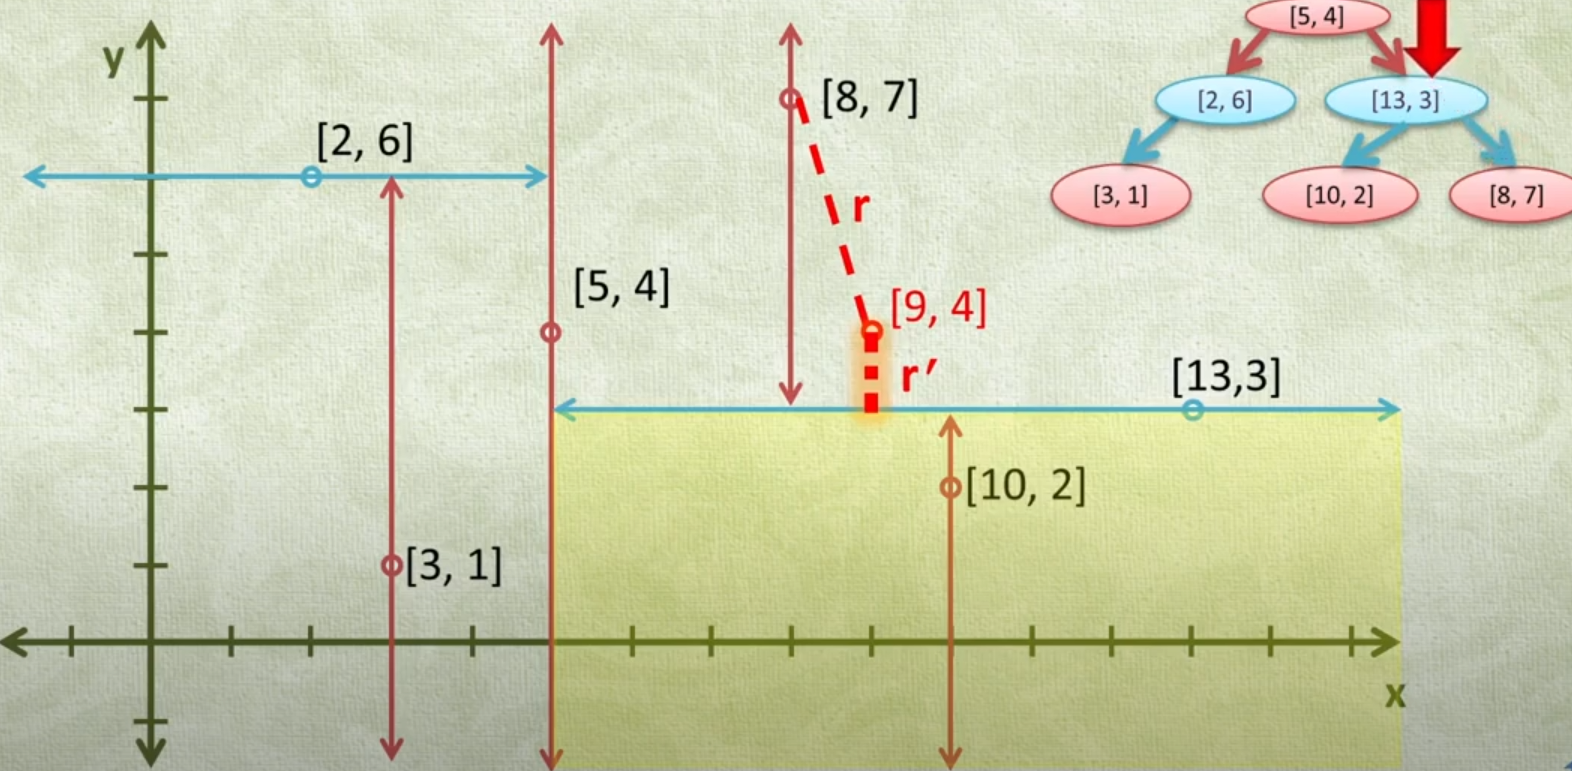
\includegraphics[width=\textwidth]{img/knn7.PNG}
                 \caption{Comparar la distancia del eje en dos valores tomando el menor para ir por la rama hija a consultar $(r, r')$}
                 \label{fig:knn7}
             \end{subfigure}
             \hfill
             \begin{subfigure}[b]{0.4\linewidth}
                 \centering
                 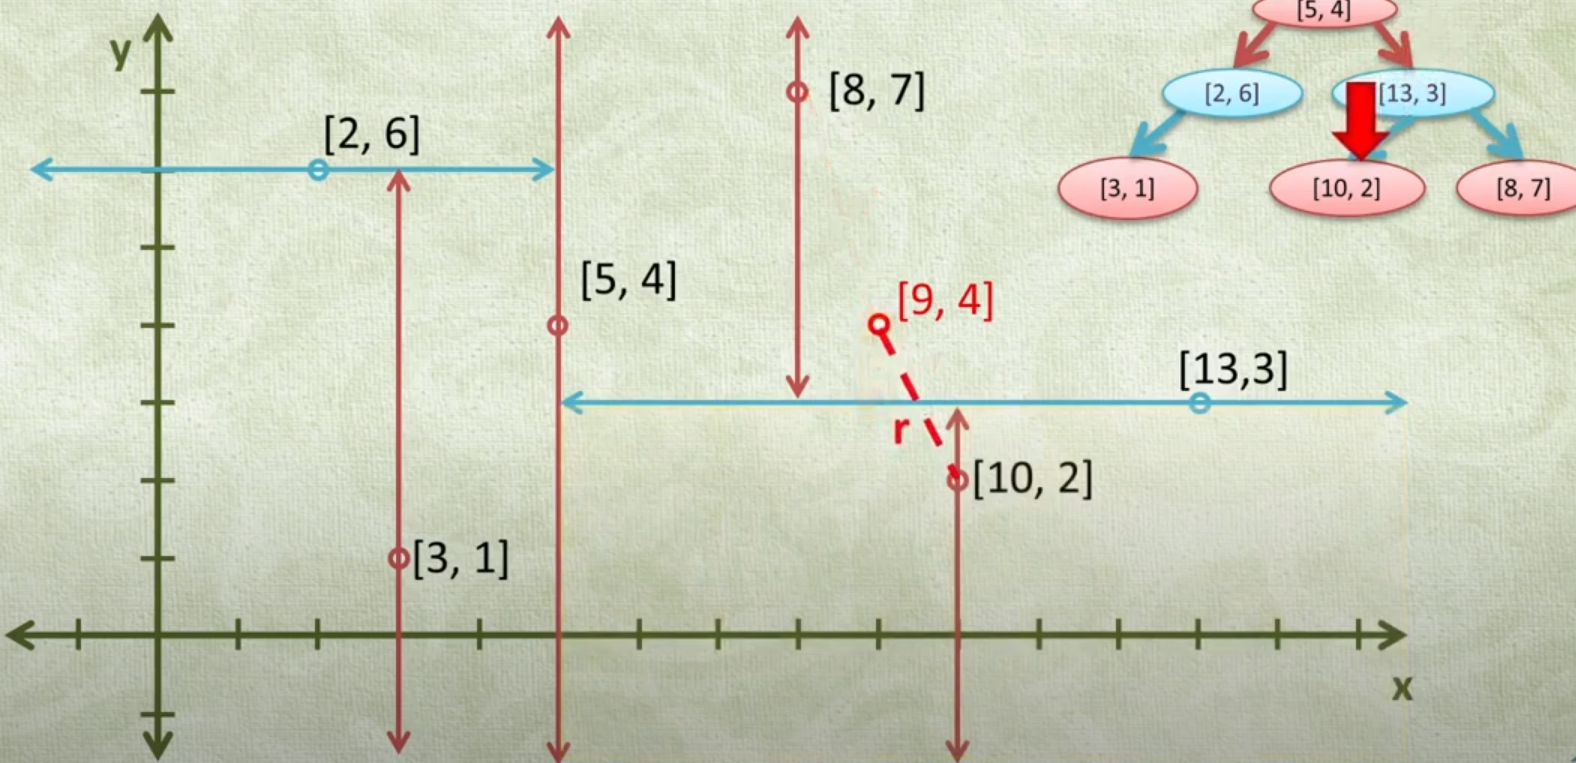
\includegraphics[width=\textwidth]{img/knn8.PNG}
                 \caption{Si el radio marcado es menor al punto elegido se actualiza el menor punto cercano}
                 \label{fig:knn8}
             \end{subfigure}
                \caption{Mediante el punto más cercano se ubica el punto a consultar}
                \label{fig:knn_2_parte}
        \end{figure}
    		
    		En el siguiente código, se mantuvo la dimensión $k=2$ solo con fines de utilizar solamente los puntos de dicha dimensión, para utilizarlo en otras implementaciones solamente debería cambiarse dicho valor por $k$. Igualmente como observación, por cada vez que se realiza el cálculo de la distancia con el punto a revisar, se ingresa a los vectores visitados el atributo distancia que no afecta a la revisión total de la $k$ dimensión.
    		
    		\lstinputlisting[language=JavaScript, firstline=160, lastline=198, caption=KNN]{code/kdtree.js}
    		
		
		\subsection{Implemente la función range query circle del KD-Tree}
		    
		    En primer lugar, se declara la función $closer\_point$ que recibe los parámetros del punto que chocará en los bordes de la consulta circular y también será reutilizada para la consulta rectangular. El resultado de realizar la comparación del punto que ingresa al rango de la consulta circular o rectangular devolviendo inversamente el resultado ya que se quiere los puntos internos respecto a la distancia de los puntos que se estén comparando.
		
    		\lstinputlisting[language=JavaScript, firstline=220, lastline=252, caption=closerPoint]{code/kdtree.js}
    		
    		La función $range\_query\_circle$ recibe los parámetros de árbol $kd-tree$, el punto céntrico del circulo consulta, el tamaño del radio, el acumulador de los puntos visitados y finalmente la profundidad del árbol que se irá acumulando. En el recorrido del cada vez que se dirige el punto céntrico respecto al radio, siempre inicia con la revisión desde el nodo raíz hacia las ramas, comparando el eje en el que se realiza la primera consulta hacia los hijos derecho o izquierdo. al tener la dirección se realiza nuevamente la consulta recursiva respecto al lado del hijo hallado, como en el caso del algoritmo KNN, si el punto respecto al radio principal es mas corto al punto del hijo donde esta apuntado la distancia, se balancea y se toma la consulta del punto que esta en otra rama y directamente se hace la comparación si la distancia calculada al punto principal es menor al radio se inserta en el arreglo consulta. finalmente actualizamos el mejor punto recursivamente. Cada consulta de hallar el punto más cercano, utilizamos la función  $closer\_point$ explicada al principio.
    		
    		\lstinputlisting[language=JavaScript, firstline=287, lastline=315, caption=rangeQueryCircle]{code/kdtree.js}
    		
    		Complementando en la consulta gráfica, para distinguir la consulta circular, en el inicio de la grafica se toma la distancia invertida del eje y para mejor visualización y distinción del centro de la figura respecto al eje. Así mismo se muestra la consulta esta englobando a los puntos que están dentro del círculo como en la figura \ref{fig:circular1}
    		
    		\begin{figure}[H]
    			\centering
    			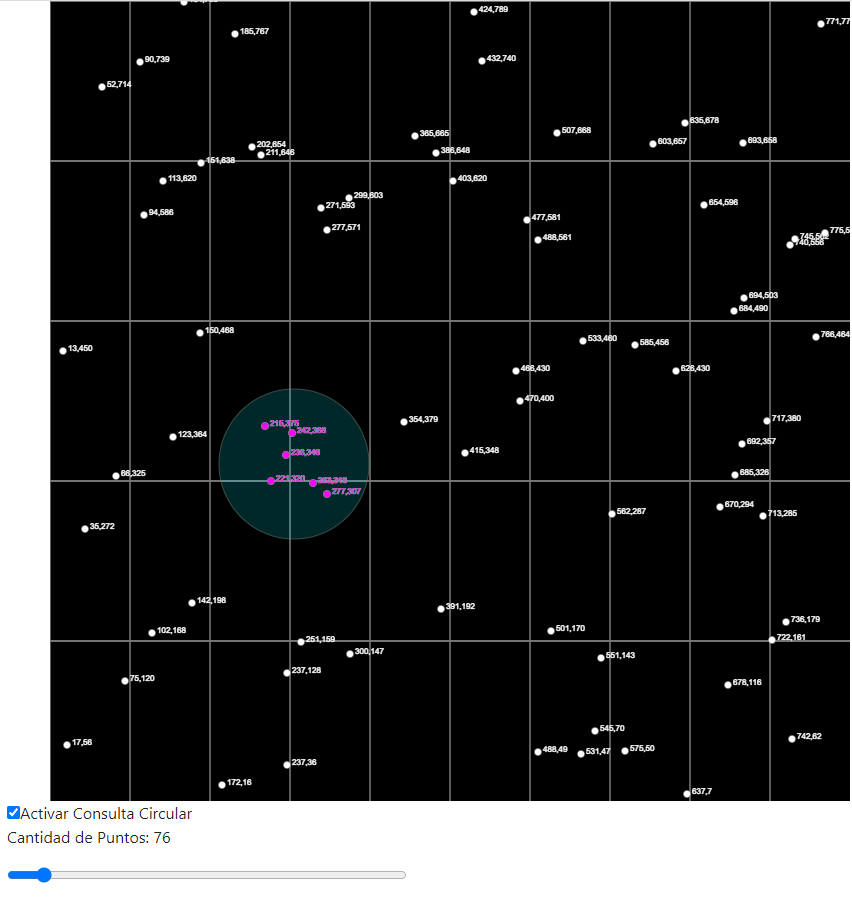
\includegraphics[scale=0.45]{img/circular1.png}
    			\caption{rangeQueryCircle}
    			\label{fig:circular1}
    		\end{figure}
    		
    	\subsection{Implemente la función range query rec del KD-Tree, esta vez el range representa un rectángulo} 
    	    La función $range\_query\_rect$ recibe los parámetros de árbol $kd-tree$, el punto céntrico del circulo consulta, el tamaño del ancho y alto en un par ordenado, el acumulador de los puntos visitados y finalmente la profundidad del árbol que se irá acumulando. Para este caso la revisión ya no se hace mediante la consulta de un radio sino, a partir de dos parámetros, ancho*2 y alto*2, igualmente la primera parte inicia la consulta desde la raíz para ir descendiendo hacia los hijos, en este caso para comparar el ingreso del punto al rectángulo se realiza una primera comparación sobre el eje en el cual se esta evaluando el punto en el nodo actual respecto al eje del rectángulo, si es menor o igual para estar incluido en la consulta inmersa del rectángulo, igualmente verificar si el punto esta dentro del rango de la distancia respecto al padre en el mismo eje para que así se pueda tomar en cuenta los puntos que no pertenecen directamente al resultado del hijo inmediato. Nuevamente se realiza la búsqueda del punto más cercano recursivamente al punto que va descendiendo en el árbol.
    	    
    	    \lstinputlisting[language=JavaScript, firstline=317, lastline=343, caption=rangeQueryRect]{code/kdtree.js}
    	    
    	    Complementando en la consulta gráfica, igualmente con la consulta circular se realizo sobre la misma cantidad de puntos en este caso se debe comparar la distancia de los ejes respecto al tamaño del rectangulo en el eje que se compara, dando como resultado los puntos que estarán inmersos dentro del rectángulo consulta \ref{fig:rectangulo1}
    		
    		\begin{figure}[H]
    			\centering
    			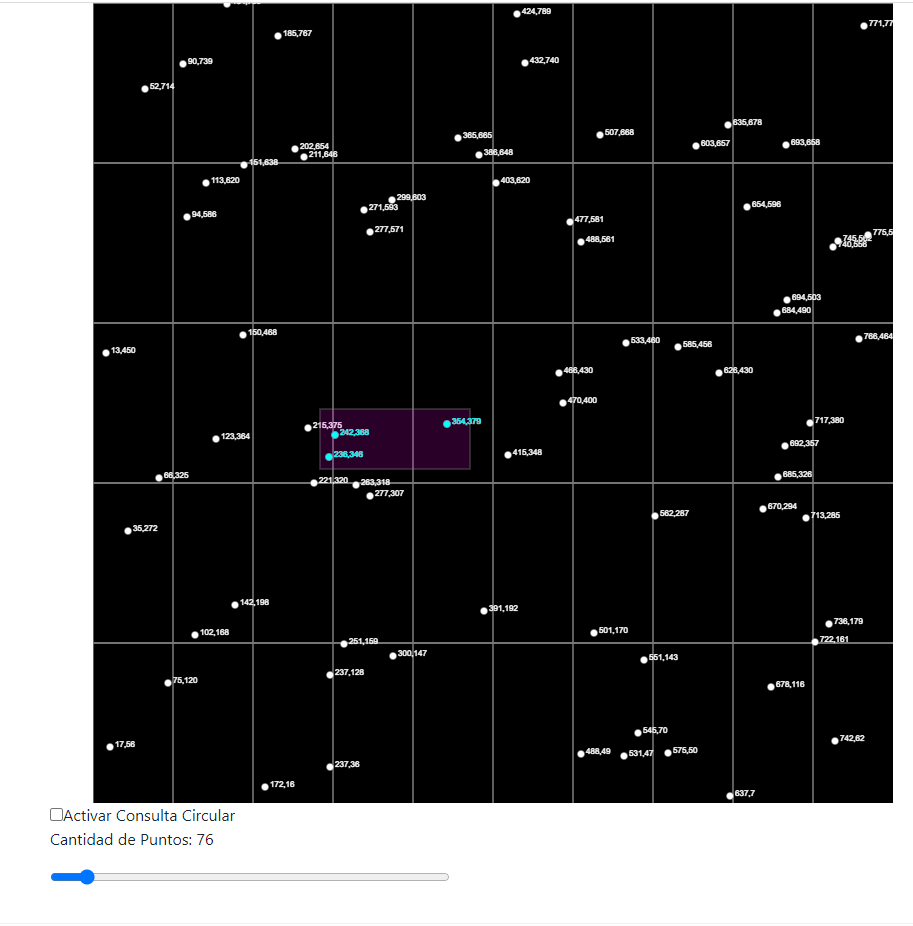
\includegraphics[scale=0.45]{img/rectangular1.png}
    			\caption{rangeQueryRect}
    			\label{fig:rectangulo1}
    		\end{figure}
    		
		
		\section{Trabajo de investigación}
		    La estructura KD-Tree es una estructura multidimensional de k dimensiones. Esta permite implementar 
		    búsquedas por similitud como $K Nearest Neighbor$ o $Closest point$. Adicionalmente, se puede
            usar esta estructura como un clasificador. Usted debe implementar este clasificador en el tema de su
            preferencia. A continuación detallamos el algoritmo:
            
            \begin{algorithm}[H]
                \begin{algorithmic}
                    \REQUIRE $X:$ training data; $y:$ objecto to be classified
                    \ENSURE Classification for $y$
                    \STATE Extract features of each sample;
                    \STATE Build KD-Tree;
                    \STATE Select KNN of $y$ in X;
                    \STATE Class(y) $\gets$ max of classes ( $k$ closest objects)
                \end{algorithmic}
                \caption{KNN Clasifier}
                \label{alg:KNNClasifier}
            \end{algorithm}
            
        \subsection{Dataset Elegido}
            Para el dataset, usamos Kaggle, que es una plataforma en la nube de Data Science más grande del mundo. Donde nos permite encontrar y publicar una amplia variedad de dataset.
            Con respecto a la elección del dataset, directamente se revisaron muchas otras opciones como el generador del buscador de películas en general, en este caso solamente se cuenta con la información de 3323 Películas en el catálogo de Netflix respecto a la cantidad presentado en el dataset $Netflix\_Movies$ \cite{kaggleNetflix} (ver figura \ref{fig:netflix1}). El dataset esta compuesto por 10 columnas(índice, nombre de la película, duración, año, género, director, actores, país, rating, ingreso en netflix), las cuales describen a las películas mencionadas anteriormente, el dataset esta en formato CSV cuyo plan inicial es realizar su lectura con ayuda de la librería Pandas de Python para realizar el análisis de preprocesamiento de la información respecto a las columnas que se tomarán como característica principal, pero para la implementación directa del vector característico se paso a un formato JSON.
            
            \begin{figure}[H]
    			\centering
    			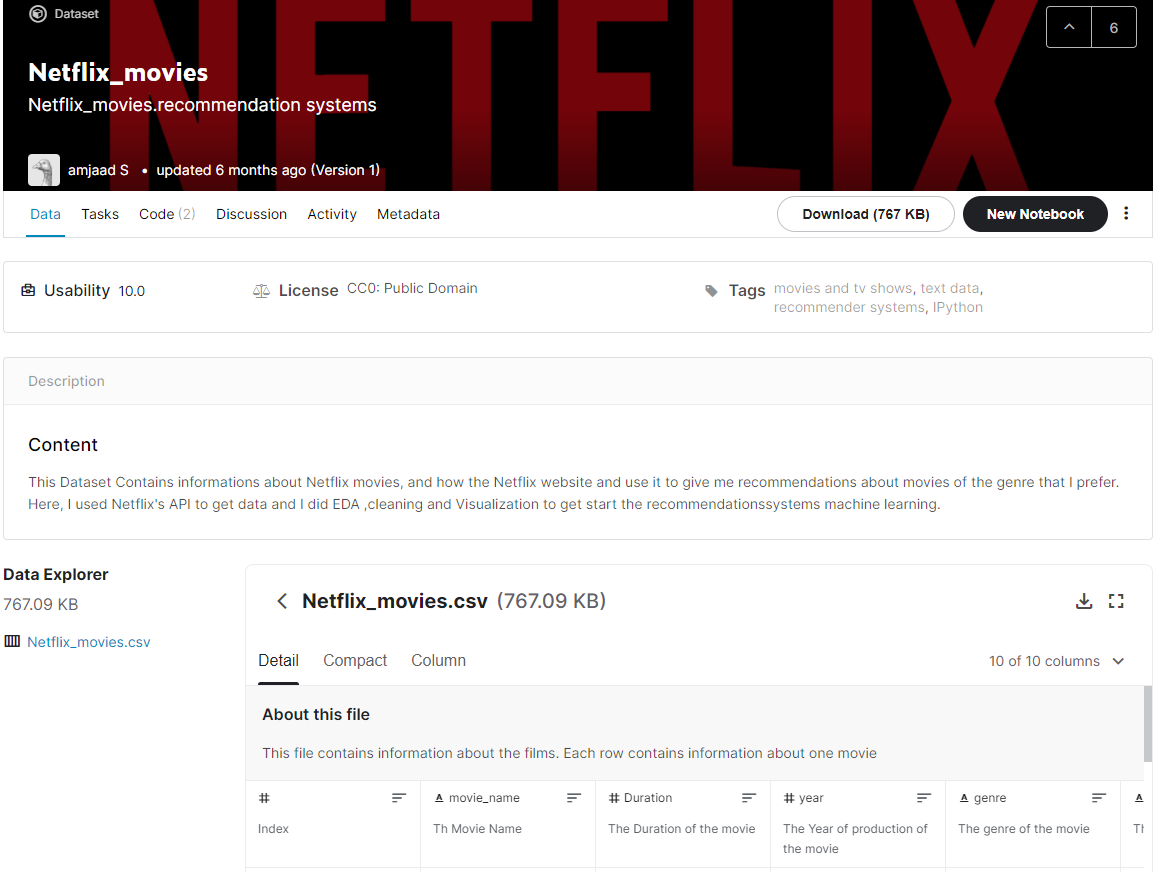
\includegraphics[scale=0.45]{img/netflix1.PNG}
    			\caption{Kaggle $Netflix\_Movies$ Dataset}
    			\label{fig:netflix1}
    		\end{figure}
    		
    	\subsection{Extracción de Características}
    	Para la extracción de características, usamos Colab, que es un servicio de Cloud que nos permite programar y ejecutar código de Python, ideal para estudiantes, científico de datos o investigador en Inteligencia Artificial.
    	Empleamos el modelo Bag of words(bolsa de palabras) es un método que se utiliza en el procesado del lenguaje para representar documentos ignorando el orden de las palabras.
    	
    	\begin{enumerate}
    	        \item Conectamos desde Colab con kaggle para importar el dataset almacenado en kaggle.
    	        \item Generamos en vector característico.
    	   Para este proceso elegimos el campo género, ya que obtuvo una dimensión de 29 en comparación con el resto de campos. Adicional a ello el vector característico final se obtuvo adicionando los 29 valores del bag of words, conjuntamente con los campos duración, año y rating, dando una dimensión de 32 valores del vector característico.
	            \begin{figure}[H]
    			\centering
    			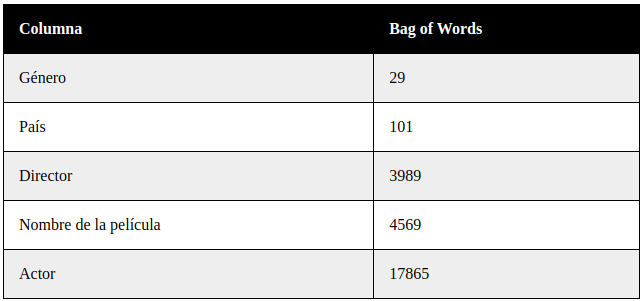
\includegraphics[scale=0.45]{img/bagofwordscomparing.png}
    			\caption{Bag of words - comparación de dimensiones}
    			\label{fig:table}
    		\end{figure}

    	         \item Exportamos el objeto generado en JSON, ya que nuestras implementaciones del kdtree y knn están implementadas en Javascript.
            	   \lstinputlisting[language=Python, firstline=1, lastline=20, caption=Objeto JSON]{code/objetoMovie.py}
    	    \end{enumerate}
    	    
     
    	
    	\subsection{Aplicación Web para las Películas}
    	    Con el objetivo de ver el funcionamiento de las operaciones del KDtree y el proceso de busqueda usando el algoritmo de Knn, se determino usar la base de caracteristicas del dataset de Netflix dado en Kaggle \url{https://www.kaggle.com/amjaads/netflix-movies}, para ello se determino usar la base de pandas\url{https://pandas.pydata.org/} para realizar las consultas y filtros sobre los datos, y puedan estos se retornados a la interfaz.
    	    
    	    En este caso la comunicación entre Python y Javascript fue dada gracias a el uso Flask \url{https://flask.palletsprojects.com/en/2.0.x/} el cual permite desarrollar una interfaz web usando Python.
    	    
    	    La parte de preparación de características se observa en la figura \ref{prepCaract}, donde extrae las 3 características numéricas (duración,anio,calificación) mas 37 características pertenecientes al genero de la película, el cual se obtuvo al aplicar el \"CountVectorizer\" sobre la columna Genero.
    	    
    	    \lstinputlisting[label={prepCaract},language=Python, firstline=74, lastline=95, caption=getFeatureVectors.py]{code/getFeatureVectors.py}
    	    
    	    La parte de consulta de los datos usando Pandas dado en la figura \ref{consultaMovies}. Por ejemplo, para un id particular de película seleccionada por el usuario y con la debida preparación de características dada en la función "buildJsonSelectedMovie", permitiendo asi devolver un dato como objeto Json para la interfaz.
    	    \lstinputlisting[label={consultaMovies},language=Python, firstline=51, lastline=57, caption=consultaMovies.py]{code/consultaMovies.py}
    	    
    	    La parte del uso del KDTree y la consulta con KNN es dada en la figura \ref{viewMovies} donde se consigue lo enviado por la consulta en Python, esto permite construir el arbol KDTree con el set completo de peliculas y realizar la consulta con la pelicula seleccionada por el usuario, ambos ya fueron vectorizados y adicionando su objeto al interior del nodo. Finalmente servir a la interfaz almacenando en el localStorage del navegador.
    	    
    	    \lstinputlisting[label={viewMovies},language=Python, firstline=68, lastline=86, caption=viewmovie.html]{code/viewmovie.html}
    	    
    	\subsection{Vista Detalle de Películas}
    	
    	Luego de realizar la búsqueda y darnos como resultado un archivo JSON necesitamos interpretar este archivo y generar un escenario de visualización de los resultados, para esto desde el backend se ha guardado el json en el almacenamiento 'local storage' el cual puede ser abierto desde el frontend, específicamente desde javascript, la sentencia que realiza esta acción es la siguiente.
    	
    	\lstinputlisting[label={viewMovies2},language=Javascript, firstline=1, lastline=18, caption=vistaLocalStorage.js]{code/vista_local_storage.js}

        Ya teniendo todos los elementos de la búsqueda, calculamos los parámetros de valoración que mostraremos de forma gráfica en barras y datos numéricos.
    
        \begin{figure}[H]
    			\centering
    			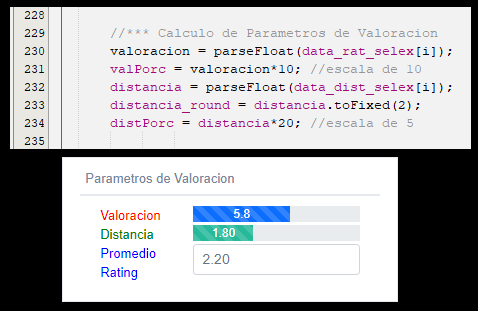
\includegraphics[scale=0.80]{img/vista_netflix_02.png}
    			\caption{Parámetros de Valoración}
    			\label{fig:netflix2}
    		\end{figure}
    		
        Finalmente las características de cada película son mostradas en paneles de visualización descendentes, cada uno contiene un video embebido de youtube que por defecto es la intro de netflix, a cada panel mostrado se le agregó un botón 'Buscar' que permite ir directamente a youtube con la búsqueda del trailer correspondiente, también se tiene un botón 'Agregar' que permite insertar la URL del tráiler en el sistema, el resultado final seria el siguiente.
	
	    \begin{figure}[H]
    			\centering
    			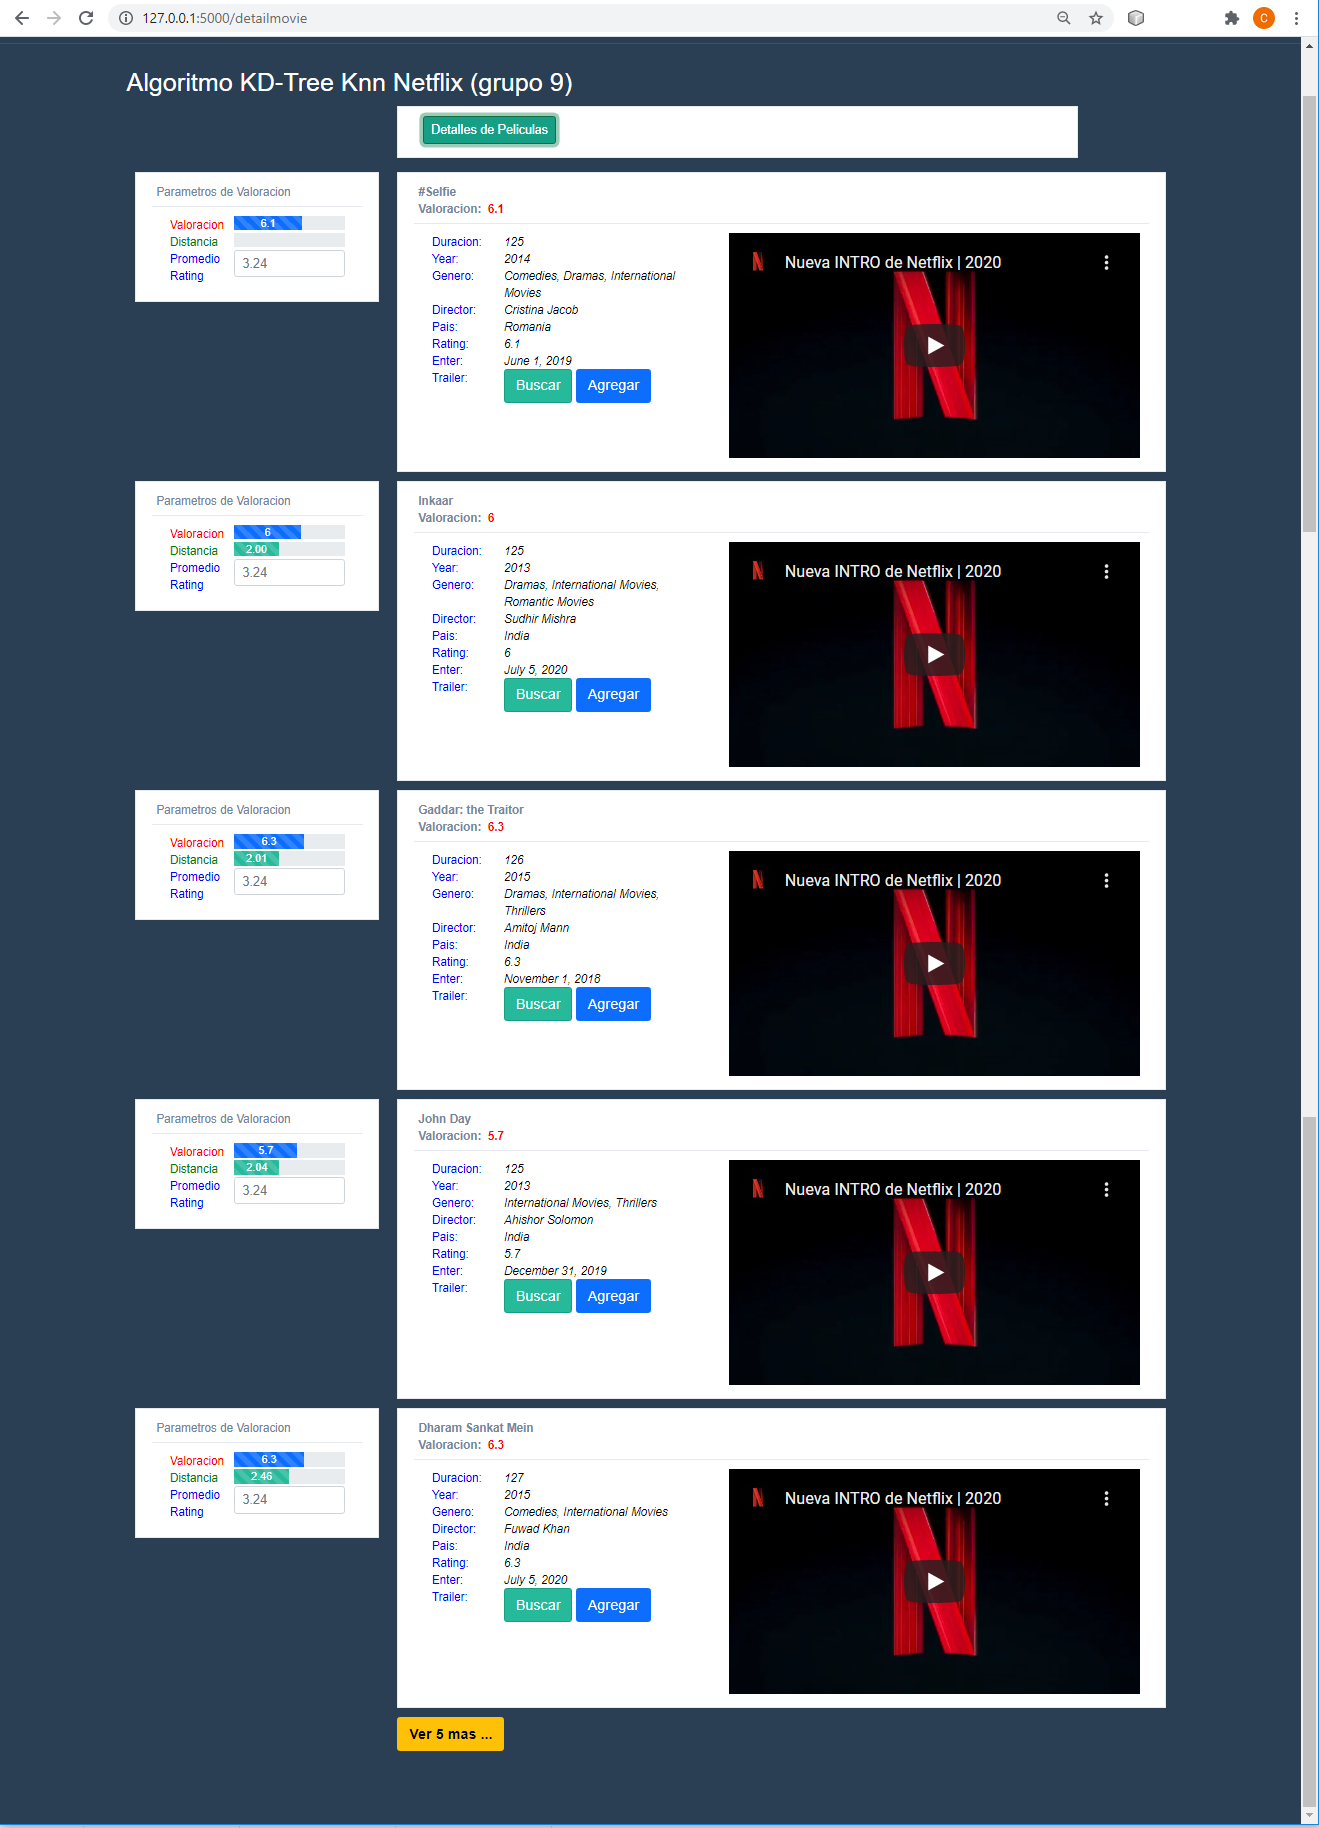
\includegraphics[scale=0.40]{img/vista_netflix_03.png}
    			\caption{Vista Gráfica KD Tree KNN Netflix}
    			\label{fig:netflix3}
    		\end{figure}
	
    \newpage
    
	\bibliographystyle{ieeetr}
    % bib stuff
    \nocite{*}
    \bibliography{biblio}
	%\bibliographystyle{apalike}
	%\bibliographystyle{IEEEtranN}
	%\bibliography{bibliography}
	
	\newpage
	
	\lstlistoflistings	
		
	
\end{document}